\chapter{Validación de la Solución Propuesta}\label{chap:3}
En el presente capítulo se presenta la validación de la herramienta desarrollada. Para ello se realizan un conjunto de pruebas funcionales, además se establece una comparación entre los resultados estadísticos obtenidos para diferentes juegos de datos. Dicho proceso parte de cómo la fase de análisis y diseño se unen para llevar a cabo el sistema propuesto.

\section{Pruebas Funcionales}
Las pruebas de software, o pruebas funcionales, son el proceso de ejecutar un sistema o componente para medir su calidad, con la intención de encontrar errores que aún no se descubren y el proceso orientado a demostrar que un programa realiza las funciones para las cuales fue construido.

El nivel de prueba que se utiliza es pruebas de sistema, donde se ejecutan en el sistema completo, buscando defectos tanto en aspectos generales como particulares del comportamiento del sistema, se prueban sus funcionalidades y las respuestas del sistema como un todo. Los tipos de pruebas que se realizan son funcionales, donde se prueba la ejecución correcta de las funcionalidades del sistema. El método que se utiliza es las pruebas de caja negra, que se llevan a cabo sobre la interfaz del software, los casos de prueba pretenden demostrar que las funciones son operativas, que la entrada se acepta de forma adecuada y que se produce un resultado correcto, así como que la integridad de la información externa. 

\subsection{Caso de Prueba: Gestionar Usuario}
\begin{figure}[h]
\centering
 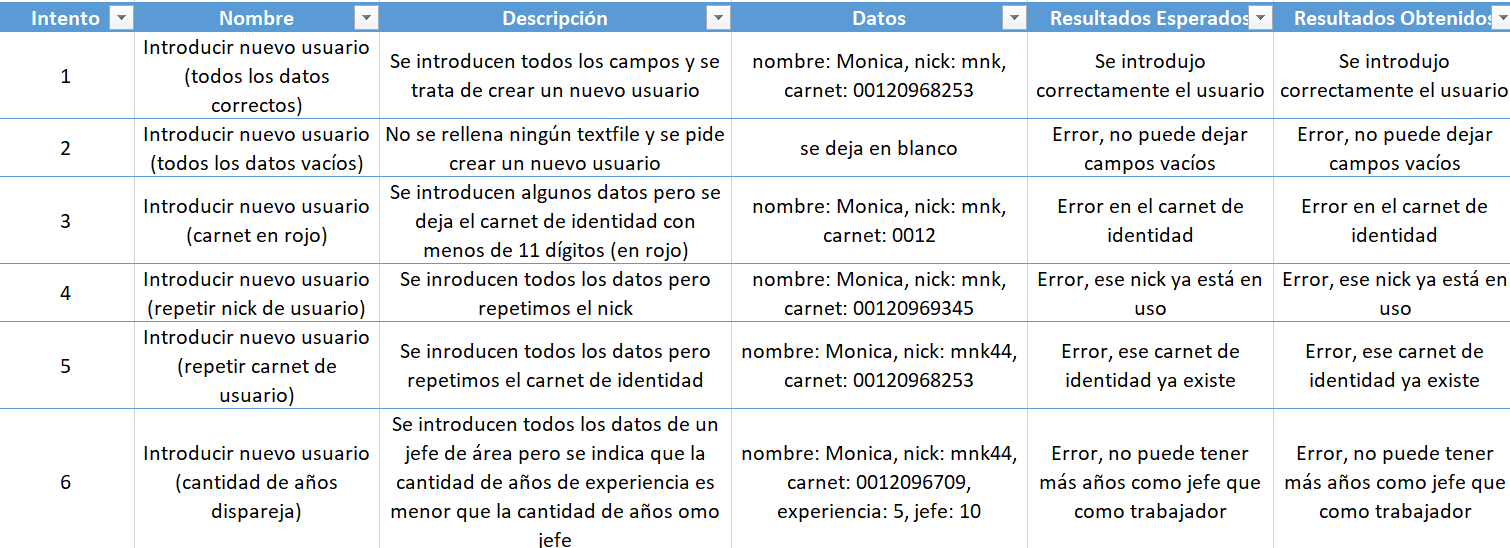
\includegraphics[width=0.8\linewidth]{imagen/introducirU.png}
 \caption{Caso de Prueba para Introducir Usuario.}
 \label{fig:introducirU} 
\end{figure}

\begin{figure}[h]
\centering
 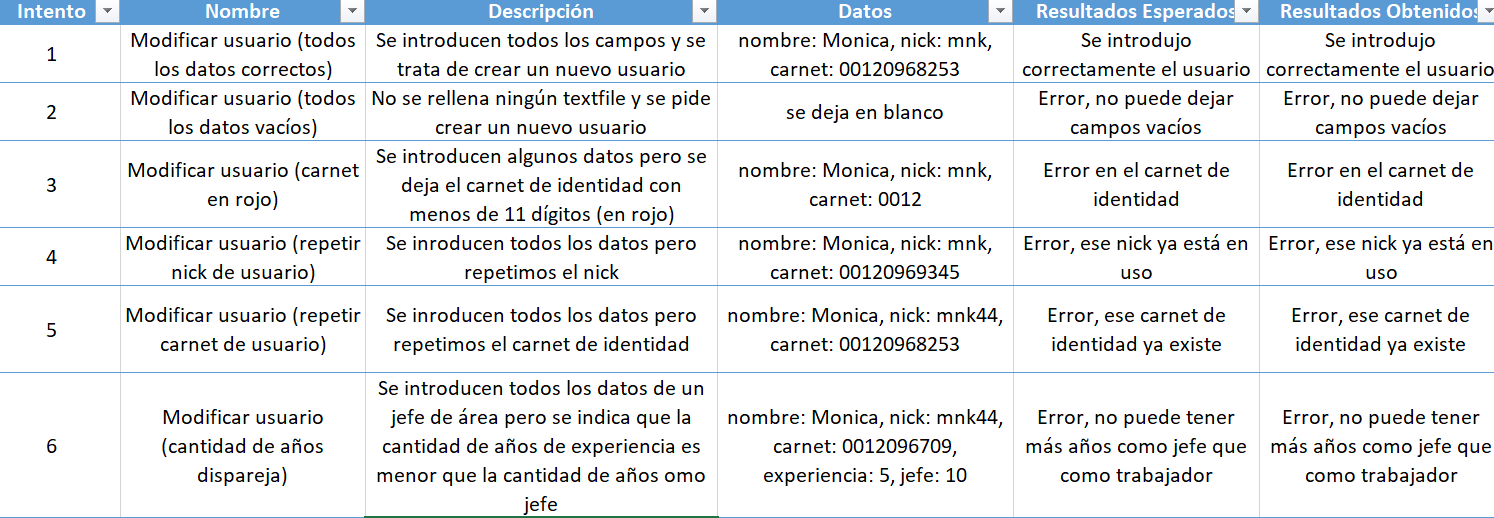
\includegraphics[width=0.8\linewidth]{imagen/modificarU.png}
 \caption{Caso de Prueba para Modificar Usuario.}
 \label{fig:modificarU} 
\end{figure}

En el caso de prueba de dormir a un usuario, la función recibe un identificador del usuario que debe dormir. No hay márgenes de error porque estos identificadores se obtienen a través de una tabla (Figura \ref{fig:img}), por lo que las pruebas con datos no fueron necesarias en este caso.

\subsection{Caso de Prueba: Gestionar Área}
\begin{figure}[h]
\centering
 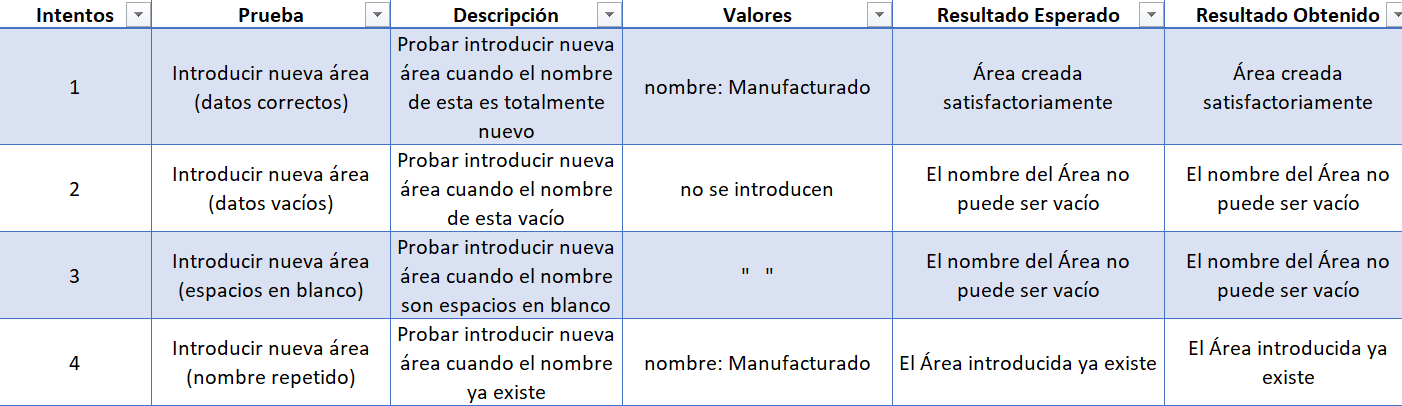
\includegraphics[width=0.8\linewidth]{imagen/introducirA.png}
 \caption{Caso de Prueba para Introducir Área.}
 \label{fig:introducirA} 
\end{figure}

\begin{figure}[h]
\centering
 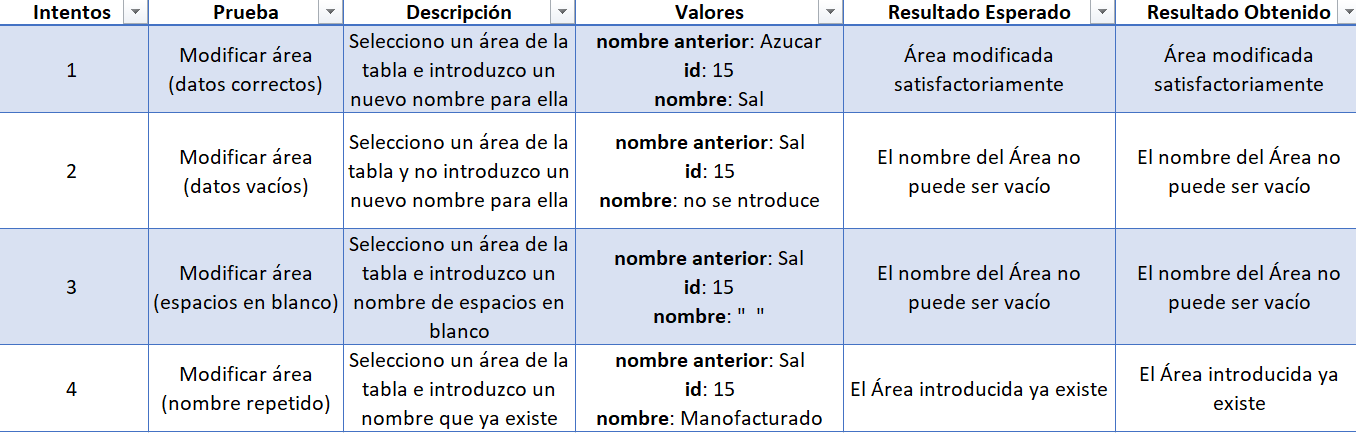
\includegraphics[width=0.8\linewidth]{imagen/modificarA.png}
 \caption{Caso de Prueba para Modificar Área.}
 \label{fig:modificarA} 
\end{figure}

\begin{figure}[h]
\centering
 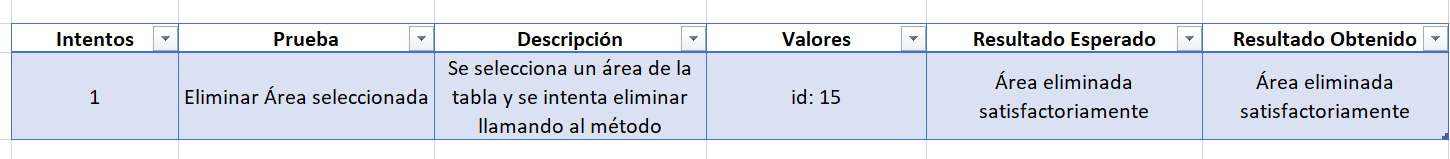
\includegraphics[width=0.8\linewidth]{imagen/eliminarA.png}
 \caption{Caso de Prueba para Eliminar Área.}
 \label{fig:eliminarA} 
\end{figure}

En el caso de prueba de eliminar un área, la función recibe un identificador del área que debe eliminar. No hay márgenes de error porque estos identificadores se obtienen a través de una tabla (Figura \ref{fig:img}), por lo que las pruebas con datos no fueron necesarias en este caso. Solo se activa el botón si el área puede ser eliminada.

\section{Análisis del Resultado de las Pruebas}
Con las pruebas realizadas se pudo comprobar el correcto funcionamiento del sistema, lo cuál resulta un logro para la investigación. También se pudo comprobar el correcto funcionamiento de las operaciones que eran necesarias modificar, tal como se propuso en un inicio.

\section{Conclusiones Parciales}
Durante este capítulo se realizaron numerosas pruebas al sistema para comprobar que los cambios realizados no afectaran sus funcionalidades. Como se pudo apreciar en los resultados obtenidos de las pruebas realizadas, los cambios no afectaron las funcionalidades, por lo que podemos afirmar que se cumplieron los objetivos de manera satisfactoria